
\textit{\textbf{Note}: Secs 1.1-1.4 in this document are an adaptation of material taken from \cite{MITcourse} (Creative Commons license BY-NC-SA 4.0). Sec. 1.5 is a translation, summary and adaptation of a chapter in \cite{ComDig2007} made by the author with permission of the co-authors. Secs. 1.1-1.4 is published under license BY-NC-SA 4.0. Sec. 1.5 cannot be published or redistributed in any form. It cannot be transformed or used partially without permission of the original authors}
\vspace{2cm}


This document introduces the concept of stochastic process and analyzes some important examples.

%%%%%%%%%%%%%%%%%%%%%%
\section{Introduction}
%%%%%%%%%%%%%%%%%%%%%%

A stochastic process (SP) is a collection of random variables $\{X_n\}$ indexed by time, $n$. Depending on the nature of the time variable, we will consider different types of SP:
\begin{itemize}
\item \textbf{Discrete-time} SP: when the time variable is a real number ($n \in \mathbb{R}$)
\item \textbf{Continuous-time} SP: when the time variable is integer ($n \in \mathbb{Z}$).
\end{itemize}

This chapter discusses discrete-time processes only. Thus, under contrary stated, all SP will be assumed to be discrete.

Depending on the range of the time variable, two types of SP will be considered:
\begin{itemize}
\item \textbf{One-side} SP: $\{X_n, n \ge 0\}$. Note that a one-side SP is a sequence of random variables.
\item \textbf{Two-side} SP: $\{X_n, n\in \mathbb{Z}\}$, the SP is defined for all integer times.
\end{itemize}

%%%%%%%%%%%%%%%
\begin{example}

Consider the one-side stochastic process $X_n$ such that, for all $n$, $X_n \in \{-n, n\}$ with $P\{X_n=n\}=P\{X_n=-n\}$ and all variables in the collection are mutually independent.

\end{example}
%%%%%%%%%%%%%

A realization of all random variables in an SP defines a signal. For this reason, we can define stochastic processes in the following alternative but equivalent form:

%%%%%%%%%%%%%%%%%%%%%%%%%%%%%%%%%%%%%%
\begin{definition}[Stochastic Process]
A discrete-time stochastic process is a probability measure over a space of (one-side or two-side) discrete-time signals.
\end{definition}

%%%%%%%%%%%%%%%
\begin{example}
\label{ex:2signals}
Consider the one-side stochastic process $X_n$ such that
\begin{align}
X_n = n, 	\quad		\text{for all } n \ge 0
\end{align}
or 
\begin{align}
X_n = -n, 	\quad		\text{for all } n \ge 0
\end{align}
with equal probabilities. Note that, the Universe set of this SP if finite, containing only two signals.

\end{example}
%%%%%%%%%%%%%


%%%%%%%%%%%%%%%%%%%%%%%%%%%%%%%%%%%%%%%%%%%%%%%%%%%%%
\subsection{Characterization of a stochastic process}

Note that the random variables defining a SP can be continuous or discrete. In general, a SP is completely characterized when we can determine the joint distribution $P(X_{n_0},X_{n_1},\ldots, X_{n_{M-1}})$ for any subset of random variables from the process. However, for many SP, the computation of these distributions is unfeasible. We will pay attention to processes satisfying different properties that simplify the characterization.


%%%%%%%%%%%%%%%%%%%%%%%%%%%%%%%
\section{Independent processes}

%%%%%%%%%%%%%%%%%%
\begin{definition}[Independent process]
A stochastic process $X_n$ is statistically independent (or, simply, independent) if all its random variables are statistically independent, that is, for any $M >0$ and any subset of $M$ random variables $X_{n_0}, X_{n_1}, \ldots, X_{n_{M-1}}$ with $n_0<n_1,\ldots < n_{M-1}$ we have
\begin{equation}
\label{def_indep}
P(X_{n_0}, X_{n_1}, \ldots, X_{n_{M-1}}) = \prod_{k=0}^{M-1} P(X_{n_k})
\end{equation}
\end{definition}
%%%%%%%%%%%%%%%%

\textbf{Note}: A quick explanation on the mathematical notation. Eq. \eqref{def_indep} should be interpreted as: the joint distribution of the set of $M$ random variables $X_{n_0}, X_{n_1}, \ldots, X_{n_{M-1}}$ is the product of the marginal distribution of each variable. Thus, for instance, the cumulative distributions gets factorized:
\begin{equation}
\label{Findep}
F_{X_{n_0}, X_{n_1}, \ldots, X_{n_{M-1}}}(x_{n_0}, x_{n_1}, \ldots, x_{n_{M-1}}) = \prod_{k=0}^{M-1} F_{X_{n_k}}(x_{n_k})
\end{equation}
for any $x_{n_0}, x_{n_1}, \ldots, x_{n_{M-1}}$ in the respective domains of the variables. If all the random variables in the process are continuous, Eq. \eqref{Findep} is equivalent to the factorization of the density functions
\begin{equation}
\label{pdf_indep}
p_{X_{n_0}, X_{n_1}, \ldots, X_{n_{M-1}}}(x_{n_0}, x_{n_1}, \ldots, x_{n_{M-1}}) = \prod_{k=0}^{M-1} p_{X_{n_k}}(x_{n_k})
\end{equation}
Also, if the random variables are discrete, this is equivalent to the factorization of the probability mass functions
\begin{equation}
\label{pmf_indep}
P_{X_{n_0}, X_{n_1}, \ldots, X_{n_{M-1}}}(x_{n_0}, x_{n_1}, \ldots, x_{n_{M-1}}) = \prod_{k=0}^{M-1} P_{X_{n_k}}(x_{n_k})
\end{equation}

In general, we will use expressions like \eqref{def_indep} instead of \eqref{Findep}, \eqref{pdf_indep}, or \eqref{pmf_indep} to state some relations between distributions, because it is simpler and encompasses all of them.

A particularly interesting case arises when all variables in the SP follow the same distribution.

%%%%%%%%%%%%%%%%%%
\begin{definition}[IID process]

A stochastic process $X_n$ is independent and identically distributed, or IID, if it is independent and all variables in the process follow the same distribution, i.e. $P(X_n)=P(X_m)$ (which implies, for instance, that $F_{X_n}(x)= F_{X_m}(x)$, for all $x$ and any $n, m$ in the time domain of the process).
\end{definition}
%%%%%%%%%%%%%%%% 

One of the simplest IID processes is the Bernoulli process.

%%%%%%%%%%%%%%%
\begin{example}
A Bernoulli process $X_n$ with parameter $p$, denoted as ${\cal B}(p)$ is an IID process given by Bernoulli random variables:
\begin{equation}
\label{SP:Bernoulli}
P_{X_n}(x) = p^x (1-p)^{1-x},  \qquad x \in \{0, 1\}
\end{equation}
\end{example}
%%%%%%%%%%%%%

(Note that Eq. \eqref{SP:Bernoulli} is equivalent to claim that $P\{X_n=1\} = p$ and $P\{X_n=0\} = 1-p$). Bernoulli and other IID processes are commonly used as building blocks of other, more complex, processes.

%%%%%%%%%%%%%%%
\begin{example}
\label{ejexp}
Figure \ref{fig:noisy_sin} shows 4 realizations of the independent stochastic process $X_n$, where each sample of the process follows a Gaussian distribution with mean and standard deviation equal to $4 \sin\left(0.05 \pi n \right)$. 
\end{example}
%%%%%%%%%%%%%

  
%%%%%%%%%%%%%
\begin{figure}[htb]
\begin{center}
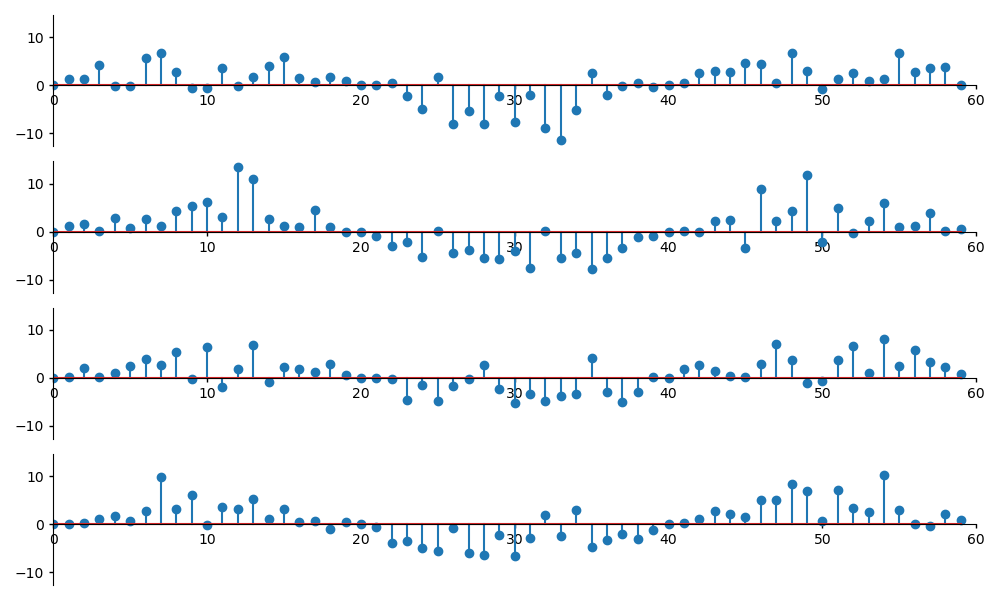
\includegraphics[width=12cm]{Figures/sp_noisy_sin.png} 
\caption{4 realizations of process $X_n$ described in example \ref{ejexp}}
      \label{fig:noisy_sin}
  \end{center}
\end{figure}
%%%%%%%%%%%%



%%%%%%%%%%%%%%%%%%%%%%
\section{Random walks}

%%%%%%%%%%%%%%%%%%
\begin{definition}[Simple random walk (SRW)]
Let $Y_n \in \{-1, 1\}$ be a one-sided IID process with $P\{Y_n= 1\}=\frac{1}{2}$. A simple random walk is defined by $X_0 = 0$ and
\begin{equation}
X_n = \sum_{k=1}^{n} Y_k,    \qquad n>0
\label{sp:srw_def}
\end{equation}
%%%%%%%%%%%%%%

\end{definition}
%%%%%%%%%%%%%%%%

Note that we can express the random variables in a SRW recursively as
 \begin{equation}
X_n = X_{n-1} + Y_n,    \qquad  n>0
\label{sp:srw_rec}
\end{equation}
Thus, a SRW is not an independent process. It is not an identically distributed process, either, since the range of the random variables in the process grows with $n$. 
\begin{align}
-n \le X_n \le n
\end{align}
Fig. \ref{fig:sp_srw} shows several realizations of the SRW. Note that the realizations are quite far from the bounds. This is because the probability that $X_n$ is close to $n$ or $-n$ vanishes for large $n$.
%%%%%%%%%%%%%%
\begin{figure}[htb]
  \begin{center}
    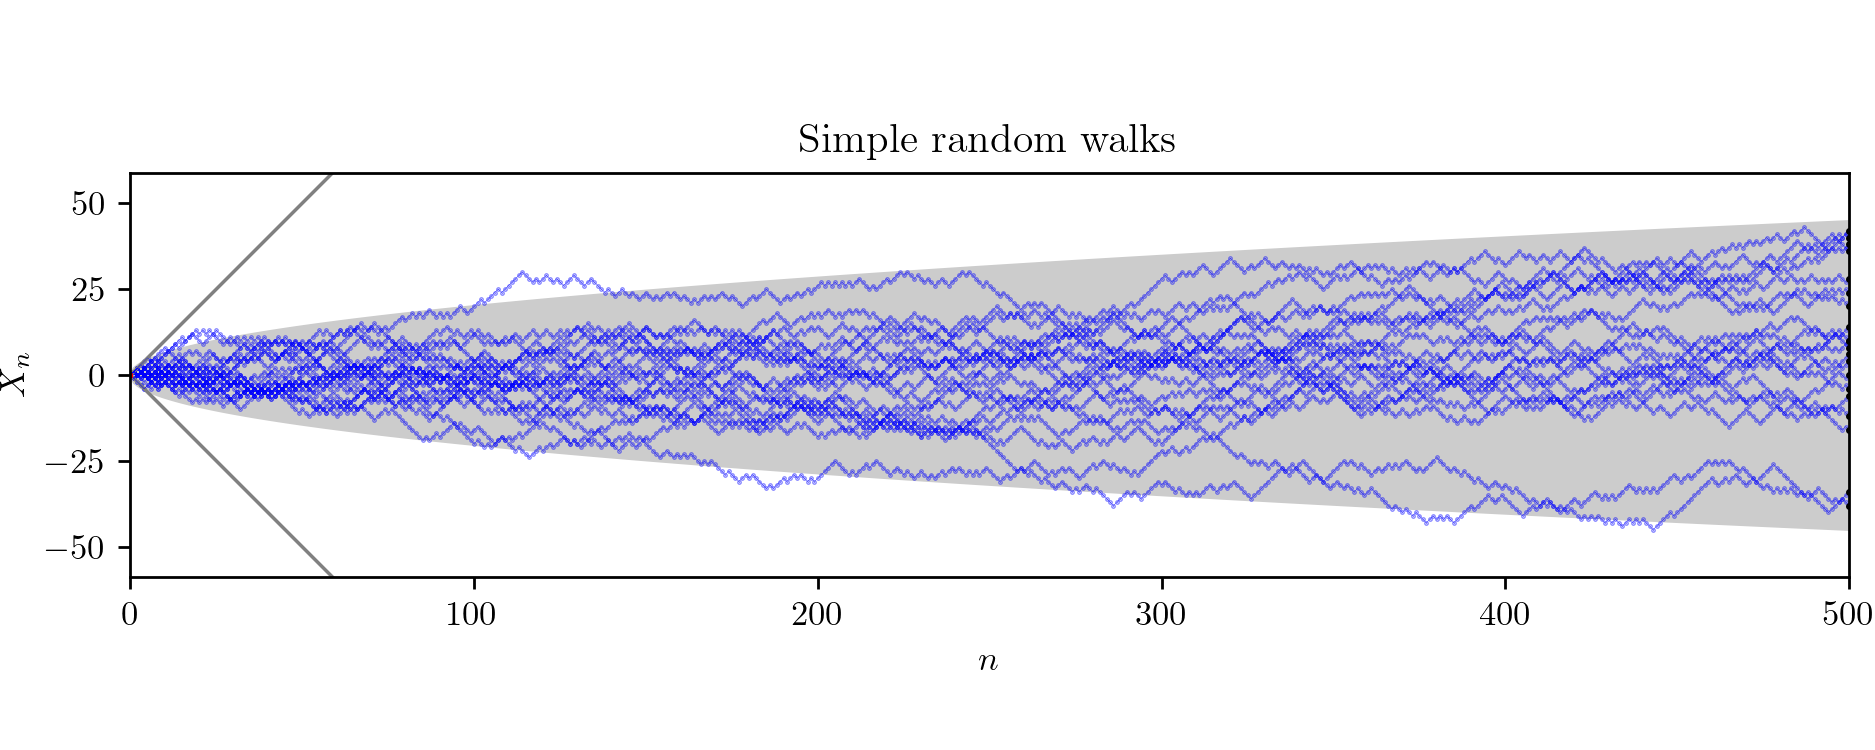
\includegraphics[width=14cm]{Figures//sp_random_walk_1d.png} 
    \caption{20 realizations of a simple random walk. The straight lines represent the boundaries of the region containing all possible trajectories. The shaded area covers two standard deviations: all trajectories tend to be inside the gray area around 95\% of the time.}
    \label{fig:sp_srw}
  \end{center}
\end{figure}
%%%%%%%%%%%%

The mean of the process is given by
\begin{align}
\mathbb{E}\{X_n\} = \sum_{k=0}^n \mathbb{E}\{Y_k\} = 0
\end{align}
and, since $Y_n$ is IID, the variance is given by
\begin{align}
\text{var}\{X_n\} = \sum_{k=1}^n \text{var}\{Y_k\} = n
\end{align}
Therefore, the standard deviation is $\sqrt{n}$ and we can expect from the process to lie between the limits $-\sqrt{n}$ and $\sqrt{n}$ most of the time. This can be expressed a bit more precisely, by noting that, since $X_n$ is the sum of $n$ independent random variable with zero-mean and bounded variance, and as a consequence of the central limit theorem, $X_n$ converges in distribution to a zero-mean Gaussian random variable with variance $n$. This implies that, after large $n$, we can expect that $|X_n| < 2\sqrt{n}$ approximately 95\% of time.

%%%%%%%%%%%%%%%%%%%%%%%%%%%%%%%%%%%%%%%%%%%
\subsection{Properties of random walks}

\begin{itemize}
\item \textbf{Independent increment} For all $0 \le n_0 \le n_1 \le n_2 \le n_3$, the random variables $X_{n_1} - X_{n_0}$ and $X_{n_3} - X_{n_2}$ are mutually independent
\item \textbf{Time invariance} For all $h \ge 1$, the SP $Z_n = X_{n+h} - X_h$ is a simple random walk.
\end{itemize}

%%%%%%%%%%%%%%%%%%%%%%%%%%%%%%%%%%%%%%%%%%%
\subsection{Stopping times}

The SRW can be used as a model of the total winning and losses of a fair game. Assume that we play a game based on repeated trials of flipping a coin. Every time the result is 'heads', we win 1 point while we loose 1 point otherwise. By taking $Y_n=1$ if the $n$-th toss is 'heads', process $X_n$ accounts for the total score after $n$ trials.

Since the SRW is zero mean, we cannot expect a positive gain after an arbitrary number of steps. One may wonder if there is a way to ensure a positive score by choosing the appropriate stopping time. Let's assume we set an upper and lower limits, $U>0$ and $-L<0$, respectively, such that, when $X_n=U$ or $X_n=-L$, we stop betting. By choosing $L$, we set the maximum loss we can tolerate, by choosing $U$, we set the gains that will make us stop playing.

We can call stopping time, $N$ to the first time where $X_N$ reaches $U$ or $-L$. Note that $N$ is a random variable, because it is a function of the random variables in the SP:
\begin{align}
N = \min\{n \mid X_n = U \text{ or } X_n = -L \} 
\end{align}

Is there a way to select $U$ and $L$ in order to expect a positive gain? To answer this question, let us compute the probability of stopping at level $U$, that is $P\{X_N=U|X_0=0\}$. Thus, defining function
$$
f(i) = P\{X_N = U | X_0 = i\}
$$
our goal is to compute $f(0)$. 

Applying the total probability theorem,
\begin{align}
f(i) =& P\{X_N = U | X_0 = i\}  \nonumber \\
     =& P\{X_1 = i+1 | X_0 = i\} P\{X_N = U | X_0 = i, X_1 = i+1\}   \nonumber \\
      &+ P\{X_1 = i-1 | X_0 = i\} P\{X_N = U | X_0 = i, X_1 = i-1\}   \nonumber\\
     =& \frac12 P\{X_N = U | X_1 = i+1\} + \frac12 P\{X_N = U | X_1 = i-1\} \nonumber\\
     =& \frac12 f (i+1) + \frac12 f(i-1)
\end{align}
Noting, also, that 
$$f(U)=1,$$
$$f(-L) = 0,$$
if we let $f(-L+1) = \alpha$ then it follows that $f(1-L + r) = \alpha r$ for all $r \le U + L$. Therefore, $\alpha = U + L$, and it follows that 
$$
f(0) = P\{X_N = U | X_0 = 0\} = \frac{L}{U + L}
$$
Thus, the gambler can increase the probability of scoring $U$ points by increasing $L$. However, this implies a higher risk to suffer large temporal losses. The expected gain becomes:
$$
\mathbb{E}\{X_N\} = U f(0) - L (1-f(0)) = 0
$$
Thus, the is no way to set the bounds $U$ and $L$ in order to expect a positive gain.

\newpage


%%%%%%%%%%%%%%%%%%%%%%%
\section{Markov Chains}

One important property of the simple random walk is that the effect of the past on the future is summarized only by the current state, rather than the whole history. In other words, the distribution of $X_{n+1}$ depends only on the value of $X_n$ and not on the whole set of values of $X_0, X_1, \ldots, X_n$. A stochastic process with such property is called a \textbf{Markov chain}.

%%%%%%%%%%%%%%%%%%
\begin{definition}[Markov property]
Let $X_n$ be a discrete-time SP that, for each $n$, takes value in some discrete set ${\cal S}$, which we call  the \textbf{state space}. We say that the SP has the Markov property if
\begin{align}
P\{X_{n+1} = i | X_n, X_{n-1}, \ldots, X_0\} = P\{X_{n+1} = i | X_n\}
\end{align}
for all $n$ in the time-domain of the process and for all $i \in {\cal S}$. 

\end{definition}
%%%%%%%%%%%%%%%% 

%%%%%%%%%%%%%%%%%%
\begin{definition}[Markov chain]

Let $X_n$ be a discrete-time SP. We say that the SP is a Markov chain (MC) if it satisfies the Markov property. 

\end{definition}
%%%%%%%%%%%%%%%% 

We will say that an MC is \textbf{finite} if ${\cal S}$ is a finite set. In this case, we usually take the elements of ${\cal S}$ as consecutive integers. For instance, for a state space with $m$ elements, we will take ${\cal S} = \{0, 1, \ldots, m-1\}$ or ${\cal S} = \{1, 2, \ldots, m\}$ under our convenience.

Note that the SRW is an MC, but it is not finite. 

Any finite MC can be described in terms of the transition probabilities
\begin{equation}
\label{SP:state_probs}
p_{ij} = P\{X_{n+1}=j| X_n=i\}
\end{equation}

All the elements of a MC model can be encoded in a transition probability matrix
\begin{align}
{\bf P} = 
\begin{pmatrix}
p_{00} & p_{01} & \ldots & p_{0,m-1}  \\
p_{10} & p_{11} & \ldots & p_{1,m-1}  \\
\vdots & \vdots & \ddots & \vdots  \\
p_{m-1,0} & p_{m-1,1} & \ldots & p_{m-1,m-1} 
\end{pmatrix}
\end{align}

Using \eqref{SP:state_probs}, it is easy to see that
\begin{align}
\sum_{j \in {\cal S}} p_{ij} = 1
\end{align}
thus, all rows in ${\bf P}$ sum up to one. For this reason, we say that ${\bf P}$ is a right-stochastic matrix. In matrix form, this property can be expressed as
\begin{align}
{\bf P}\mathbb{1}_m = \mathbb{1}_m
\label{sp:psum1}
\end{align}
where $\mathbb{1}_m$ is an all-ones vector with dimension $m$.

Note that, in general, the transition probabilities $p_{ij} $ (and, thus, the transition matrix) may change with time. However, the case of constant probabilities is particularly interesting.

%%%%%%%%%%%%%%%%%%
\begin{definition}[Homogeneous Markov Chain]
A markov chain $X_n$ is homogeneous if the transition probabilities do not depend on time, that is.
\begin{align}
P\{X_{n+1}=j| X_n=i\} = P\{X_{m+1}=j| X_m=i\},   \qquad i \in {\cal S},\quad  j \in {\cal S} 
\end{align}
for any $m$ and $n$ in the time domain of the process.
\end{definition}
%%%%%%%%%%%%%%%%


%%%%%%%%%%%%%%%
\begin{example}[Two-state machine]
A machine can be either working or broken on a given day. If it is working, it will break down in the next day with probability 0.01, and will continue working with probability 0.99. If it breaks down
on a given day, it will be repaired and be working in the next day with probability 0.8, and will continue to be broken down with probability 0.2. We can model this machine by a Markov chain with two states: working, and broken down. The transition probability matrix is given by
$$
\begin{pmatrix}
0.99 & 0.8 \\
0.01 & 0.2
\end{pmatrix}
$$
\end{example}
%%%%%%%%%%%%%

%%%%%%%%%%%%%%%
\begin{example}[SRW]
A simple random walk is an example of an MC. However, there is no transition probability matrix associated with the simple random walk since the sample space is infinite.
\end{example}
%%%%%%%%%%%%%

%%%%%%%%%%%%%%%%%%%%%%%%%%%%%
\subsection{Transition graph}

The transition probability matrix of a given homogeneous MC can be  represented by a directed graph, whose nodes are the states, and and edges from node $i$ to node $j$ represents a transition from state $i$ to state $j$ with nonzero probability. The weight of the edge is the transition probability.

%%%%%%%%%%%%%%%
\begin{example}\label{sp:MC3ex}
The transition graph of an MC given by state space ${\cal S} = \{0, 1, 2\}$ and transition probability matrix
\begin{align}
\label{sp:MC3example}
{\bf P} = \begin{pmatrix}
0.4 & 0.2 & 0.4 \\
0   & 1   & 0 \\
0   & 0   & 1 
\end{pmatrix}
\end{align}
is shown in Figure \ref{fig:sp_mc}.
\end{example}
%%%%%%%%%%%%%

%%%%%%%%%%%%%%
\begin{figure}[htb]
  \begin{center}
    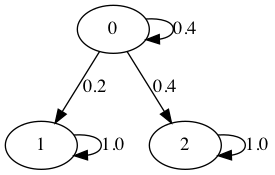
\includegraphics[width=4cm]{Figures/MC0_markov_chan_graph.png} 
    \caption{The transition graph for the markov chain given by \eqref{sp:MC3example}}
    \label{fig:sp_mc}
  \end{center}
\end{figure}
%%%%%%%%%%%%

%%%%%%%%%%%%%%%%%%%%%%%%%%%%%%%%
\subsection{State probabilities}

The transition probability matrix is useful to compute any probabilities about the state of the process at any given time. For instance, the $n$-th step transition probabilities, defined as $r_{ij}(n) = P\{X_n = j | X_0 = i\}$ can be computed recursively, by applying the total probability theorem, as
\begin{align}
r_{ij}(n) 
	&= \sum_{k \in {\cal S}} P\{X_n = j | X_{n-1} = k,  X_0 = i\} P\{X_{n-1} = k | X_0 = i\}  
	 = \sum_{k \in {\cal S}} r_{ik}(n-1) p_{kj},  \qquad n > 1 
\label{sp:mc_rij_rec}	
\end{align}
Note that $r_{ij}(1)= p_{ij}$. 

Defining the $n$-step transition probability  matrix ${\bf R}_n$ as the matrix with components $r_{ij}(n)$, the recurrent relation \eqref{sp:mc_rij_rec} can be written in matrix form as
\begin{align}
{\bf R}_n = {\bf R}_{n-1}{\bf P}
\end{align}
and, noting that ${\bf R}_1={\bf P}$, we get
\begin{align}
{\bf R}_n = {\bf P}^n
\label{sp:mc_Rn_rec}	
\end{align}

Using these relations we can compute the state probabilities at any given time, given the initial state or the initial state probabilities.

For instance, let ${\bf q}_n$ be the state probability vector at time $n$, that is
\begin{align}
q_{n,i} = P\{X_n = i\},    \quad n \ge 0, \quad {i \in {\cal S}}
\end{align}
then we can express the state probability vector at time $n$ as a function of the initial state probabilities using \eqref{sp:mc_Rn_rec} as
\begin{align}
q_{n,j} &= P\{X_n = j\} 
         = \sum_{i \in {\cal S}} P\{X_n = j | X_0 = i\} P\{X_0 = i\} \nonumber\\
        &= \sum_{i \in {\cal S}}  r_{ij}(n) P\{X_0 = i\}
\end{align}
which, in vector form, can be computed as
\begin{align}
{\bf q}_n = {\bf R}_n^\intercal {\bf q}_0 = \left({\bf P}^\intercal\right)^n {\bf q}_0
\end{align}

%%%%%%%%%%%%%%%%%%%%%%%%%%%%%%%%%%%%
\subsection{Stationary distribution}

%%%%%%%%%%%%%%%%%%
\begin{definition}[Stationary distribution]
A stationary distribution of an MC is a probability distribution over the state space ${\cal S}$ (where $P\{X_0=j\} = \pi_j$) such that
\begin{equation}
\label{sp:mc_stat_def}
{\bf P}^\intercal \bm{\pi} = \bm{\pi}
\end{equation}

\end{definition}
%%%%%%%%%%%%%%%%%%

%%%%%%%%%%%%%%%
\begin{example}
Let ${\cal S} = \mathbb{Z}_m$ and $X_0=0$. Consider the MC $X_n$ such that $X_{n+1}=(X_n+1) \mod m$ with probability $\frac12$ and $X_{n+1} = (X_n-1) \mod  m$ with probability $\frac12$.

The stationary distribution of this MC is $\pi_i = \frac1m$.
\end{example}
%%%%%%%%%%%%%

Note that the vector $\bm{\pi} = (\pi_1, \pi_2, \ldots , \pi_m)^\intercal$ is an eigenvector of ${\bf P}^\intercal$ with eigenvalue 1. Hence the following theorem can be deduced from the Perron-Frobenius theorem.

%%%%%%%%%%%%%%%
\begin{theorem}
If $p_{ij} > 0$ for all $i, j \in {\cal S}$, then there exists a unique stationary distribution of the system. 

Moreover, if ${\bf r}_i(n)$ is the state conditional probability vector with components $r_{ij}(n)$, $j \in {\cal S}$ (i.e., the values in the $i$-th row of ${\bf R}_n$),
\begin{align}
\lim_{n \rightarrow \infty} {\bf r}_i(n) = \bm{\pi}, \qquad \forall i, j \in {\cal S}
\end{align}
\end{theorem}
%%%%%%%%%%%%%

A corresponding theorem is not true if we consider infinite state spaces.

Finite Markov chains can be shown to have at least one stationary distribution. However, if at least one of the transition probabilities is zero, the behavior of the process may depend on the topology of the transition graph:

%%%%%%%%%%%%%%%
\begin{itemize}
\item The stationary distribution may be not unique.
\item The limiting distributions $\lim_{n \rightarrow \infty} {\bf r}_i(n)$ may depend on $i$.
\end{itemize}

%%%%%%%%%%%%%%%
\begin{example}

The MC in example in \ref{sp:MC3ex} has at least two limiting distributions: $\bm{\pi}_A = (0, 1, 0)^\intercal$ and $\bm{\pi}_B = (0, 0, 1)^\intercal$. Also, any convex combination of them $\bm{\pi} = \alpha \bm{\pi}_A + (1-\alpha) \bm{\pi}_B$, with $0\le \alpha \le 1$ is a stationary distribution. 

The limiting distributions depend on the initial state: is is easy to verify that 
\begin{align}
\lim_{n \rightarrow \infty} {\bf r}_i(n) &= (0, 0, 1)  \\
\lim_{n \rightarrow \infty} {\bf r}_i(n) &= (0, 1, 0)  \\
\lim_{n \rightarrow \infty} {\bf r}_i(n) &= \left(0, \frac13, \frac23 \right)
\end{align}

\end{example}
%%%%%%%%%%%%%

%%%%%%%%%%%%%%%%%%%%%%%%%%%%%%%%%%%%%%%%%%%%%%%%%%
\subsection{Computing the stationary distribution}

In general, the stationary distribution are all the solution of the set of equations \eqref{sp:mc_stat_def} and the probabilistic constraint $\mathbb{1}^\intercal {\bf p} =1$, that is
\begin{align}
\label{sp:mc_stat_eq}
\begin{pmatrix}
{\bf P}^\intercal - {\bf I}  \\
\mathbb{1}^\intercal   
\end{pmatrix}
\bm{\pi} = 
\begin{pmatrix}
0 \\ \vdots \\ 0 \\ 1
\end{pmatrix}
\end{align}

The system of linear equations given by \eqref{sp:mc_stat_eq} is consistent (it has at least one solution) but overdetermined, because the left matrix has $m+1$ rows but only $m$ columns. In fact, using \eqref{sp:psum1}, it is easy to see that 
\begin{equation}
\mathbb{1}_m^\intercal \left({\bf P}^\intercal - {\bf I}\right)  = {\bf 0}
\end{equation}
so that the rank of ${\bf P}^\intercal - {\bf I}$ is at most $m-1$. Thus, we can remove one of the rows in the matrix (any one of them) to solve the system.

\newpage


%%%%%%%%%%%%%%%%%%%%%%%%%%%%%%
\section{Stationary Processes}
%%%%%%%%%%%%%%%%%%%%%%%%%%%%%%

\textit{[\textbf{Note}: This section is copywrighted. It cannot be published or redistributed in any form. It cannot be transformed or used partially without permission of the original authors]}
\vspace{2cm}

Stationarity refers to the time invariance of some statistical properties of a stochastic process. We have already seen some forms of time invariance in the previous sections: 

\begin{itemize}
\item The homogeneity of Markov chain, $X_n$, which implies the time invariance of the conditional probabilities: $P(X_n|X_m) = P(X_{n+k}|X_{m+k})$, for any $k \ge 0$, $n \ge m \ge 0$. 
\item The time invariance of IID processes, which implies the invariance of the single-variable marginal distributions, $P(X_{n+k}) = P(X_n)$ for any $h>0$
\item The time invariance property of a SRW, which implies that $P(X_{n+h}-X_h) = P(X_n)$.
\end{itemize}

In this section we introduce two forms of stationarity which are particularly interesting in statistical signal processing applications. In its more restrictive form, stationarity implies the invariance of all joint distributions.

%%%%%%%%%%%%%%%%%%%%%%%%%%%%%%%%%%%%%%
\subsection{Strict-Sense Stationarity}
\label{sec:Stationarity}

%%%%%%%%%%%%%%%%%%
\begin{definition}[Strict-Sense Stationarity]
A stochastic process is said to be Strict-Sense Stationary (or simply SSS) if all joint distributions are invariant to a time shift, that is, for any $N>0$, any sampling times $n_0, \ldots, n_{N-1}$ (in the time domain of the process) and any time shift $m > 0$, 
\begin{equation}
\label{ec:strict}
P(X_{n_0},X_{n_1}, \ldots, X_{n_{N-1}}) = P(X_{n_0 + m}, X_{n_1 +m}, \ldots, X_{n_{N-1}+m})
\end{equation}
\end{definition}
%%%%%%%%%%%%%%%%

Thus, if a stochastic process $X_n$ is SSS, the process $Y_n = X_{n+m}$ defines the same probability measure over the signal space. 

%%%%%%%%%%%%%%%
\begin{example}[Bernoulli process]
\label{Ex:BinaryRandom}

A Bernoulli process, ${\cal B}(p)$ given by \eqref{SP:Bernoulli} is IID, thus, its joint probability mass function has the form
\begin{equation}
P_{X_{n_0},\ldots,X_{n_{N-1}}}(x_0,\ldots,x_{N-1})
    = \prod_{i=0}^{N-1} p^{x_i} (1-p)^{1-x_i}
    = p^{\sum_{i=0}^{N-1}x_i} (1-p)^{N - \sum_{i=0}^{N-1}x_i}
\label{ec:PbOrderN}
\end{equation}
which does not depend on $n_0, \ldots, n_{N-1}$. Thus, the Bernoulli process is SSS. 
 
\end{example}
%%%%%%%%%%%%%

In general, all IID processes are SSS. On the contrary, independent but not identically distributed processes are not SSS. This is the case of non-constant deterministic process, as the following example shows

%%%%%%%%%%%%%%%
\begin{example}[Deterministic process]
\label{Ex:SPdeterministic}

Consider the deterministic process given by $X_n = 2 n$ (with probability 1), that is, for each time $n$, $X_n$ is a discrete random variable with PMF
\begin{equation}
P_{X_n}(k) = \delta[k-2 n]
\end{equation}
Since $P_{X_n}(k)$ depends on $n$, $X_n$ is not SSS.

\end{example}
%%%%%%%%%%%%%

In general, strict stationarity is difficult to check and overly restrictive, and weaker forms of stationarity are more interesting. In the following, we will focus in the invariance of first and second order statistics\footnote{In this document, first and second order statistics refer to the expected value of polynomial functions of a random variable up to degree 2, that, it, the mean, the correlation and other related statistics, like the covariance. This should not be confused with the so called "order statistics".}


%%%%%%%%%%%%%%%%%%%%%%%%%%%%%%%%%%%%
\subsection{First and Second-Order Statistics}
\label{sec:CaracterizProcStoc}

In order to define wide-sense stationarity, we will first define some first and second-order statistics of stochastic processes. We will assume, in general, stochastic processes which can take complex values:


%%%%%%%%%%%%%%%%%%
\begin{definition}[First and second order statistics]
Given stochastic process $X_n$ we define the following statistics:

\begin{itemize}
\item \textbf{Mean}:
\begin{equation}\label{ec:DefMediaProcCont}
  \mu_X[n] = \mathbb{E}\{X_n\}
\end{equation}
\item \textbf{Autocorrelation}:
\begin{equation}
r_X[n_1,n_2] = \mathbb{E}\{X_{n_1}X^*_{n_2}\}
\label{ec:autocorr}
\end{equation}
\item \textbf{Cross correlation}
\begin{equation}
r_{XY}[n_1,n_2] = \mathbb{E}\{X_{n_1}Y^*_{n_2}\}
\end{equation}
\end{itemize}

Given stochastic processes $X_n$ and $Y_n$ with means $\mu_X[n]$ and $\mu_Y[n]$, we define the following joint statistics:
\begin{itemize}
\item \textbf{Cross covariance} between $X_n$ and $Y_n$
\begin{equation}
c_{XY}[n_1,n_2] = \mathbb{E}\{(X_{n_1}- \mu_X[n_1]) (Y_{n_2}-\mu_Y[n_2])^*\}
\end{equation}
\item \textbf{Autocovariance}
\begin{equation}
c_X[n_1,n_2] = \mathbb{E}\{(X_{n_1}- \mu_X[n_1]) (X_{n_2}- \mu_X[n_2])^*\}
\end{equation}
\end{itemize}
\end{definition}
%%%%%%%%%%%%%%%%

Note that $c_X[n, n]$ is the variance of $X_n$. It is easy to verify that the autocovariance and the autocorrelation are related by
\begin{equation}
c_X[n_1,n_2] = r_X[n_1,n_2] - \mu_X[n_1] \mu_X^*[n_2]
\label{SP:cx_vs_rx}
\end{equation}

%%%%%%%%%%%%%%%
\begin{example}[Bernoulli process]
\label{Ex:BinaryRandom2}

For a Bernoulli process, ${\cal B}(p)$, using \eqref{SP:Bernoulli} we get
\begin{equation}
\mu_X[n] = \mathbb{E}\{X_n\} = p,
\label{ec:Mean_b}
\end{equation}
also 
\begin{align}
r_X[n_1,n_2] 
	&= \mathbb{E}\{X_{n_1}X_{n_2}\}
     = \left[\begin{array}{ll}
        \mathbb{E}\{X_{n_1}^2\}                     & \mbox{ if } n_1 = n_2 \\
        \mathbb{E}\{X_{n_1}\} \mathbb{E}\{X_{n_2}\} & \mbox{ if } n_1\neq n_2
       \end{array}
      \right]
     = \left[\begin{array}{ll}
        p   & \mbox{ if } n_1 = n_2 \\
        p^2 & \mbox{ if } n_1\neq n_2
      \end{array}
    \right]    \nonumber\\
    &= p^2 + p(1-p) \delta[n_1-n_2]
\label{ec:r_b}
\end{align}
and $c_X[n_1,n_2] = r_X[n_1, n_2]$.

\end{example}
%%%%%%%%%%%%%

%%%%%%%%%%%%%%%
\begin{example}[Deterministic process]
\label{Ex:SPdeterministic2}

Consider the deterministic process in Example \ref{Ex:SPdeterministic}, we have
\begin{equation}
\mu_X[n] = \mathbb{E}\{X_n\} = \mathbb{E}\{2n\} = 2n,
\end{equation}
\begin{equation}
r_X[n_1,n_2] = \mathbb{E}\{X_{n_1} X_{n_2}\} = \mathbb{E}\{4 n_1 n_2\} = 4 n_1 n_2
\label{RxDeterministic}
\end{equation}
and, using \eqref{SP:cx_vs_rx}
\begin{equation}
c_X[n_1,n_2] = 0
\label{RxDeterministic}
\end{equation}

\end{example}
%%%%%%%%%%%%%


%%%%%%%%%%%%%%%
\begin{example}
\label{Ex:SimpleProc}
Consider the stochastic process $X_n$ given by
\begin{equation}
X_n = (1 + n^2) Y 
\end{equation}
where $Y$ is a real Gaussian random variable with zero mean and unit variance. 

The mean and the autocorrelation of the process can be easily calculated as
\begin{equation}
\mu_X[n] = \mathbb{E}\left\{Y\right\} \cdot (1 + n^2) = 0
\end{equation}
\begin{equation}
r_X(n,m) = \mathbb{E}\{X_n X_m\}
         = (1 + n^2) \cdot (1 + m^2) \cdot \mathbb{E}\left\{Y^2\right\} 
         =  (1 + n^2) \cdot (1 + m^2) 
\label{ec:autocorr2}
\end{equation}
Since $X_m$ has zero mean, the autocovariance is equal to the autocorrelation, and the variance is
\begin{equation}
\sigma_X^2[n] = r_n[n, n] = \left(1 + n^2\right)^2
\end{equation}

\end{example}
%%%%%%%%%%%%%

%%%%%%%%%%%%%%%
\begin{example}[Simple Random Walk]
\label{Ex:RandomWalk}

For the SRW $X_n$ given by \eqref{sp:srw_def}, the value of the process at any time $n$ depends on the value of a set of $n$ random variables ($Y_1,\ldots Y_n$). We have seen that the process is zero-mean with variance $n$. The autocorrelation (equal to the autocovariance) can be computed as
\begin{align}
r_X[n_1, n_2] 
	&= \mathbb{E}\{X_{n_1}X_{n_2}\}  
	 = \sum_{k=1}^{n_1} \sum_{\ell=0}^{n_2} \mathbb{E}\{Y_k Y_\ell\}  
	 = \sum_{k=1}^{n_1} \sum_{\ell=0}^{n_2} \delta[k - \ell]   \nonumber\\
	&= \min(n_1, n_2)
\label{eq:rx_srw}
\end{align}

\end{example}
%%%%%%%%%%%%%


%%%%%%%%%%%%%%%%%%%%%%%%%%%%%%%%%%%%
\subsection{Wide-Sense Stationarity}
\label{sec:CaracterizProcStoc}

We are ready to define a weaker form of stationarity:

%%%%%%%%%%%%%%%%%%
\begin{definition}[Wide-Sense Stationarity]
A two-sided stationary process is Wide-Sense Stationary (or simply WSS) if its mean and autocorrelation functions are invariant to a time shift, that is, for any integers $n, n_1, n_2$ and any time shift $m \in \mathbb{Z}$,
\begin{equation}
\mu_X[n] = \mu_X[n+m]
\end{equation}
and
\begin{equation}
r_X[n_1,n_2] = r_X[n_1 + m, n_2 + m]
\end{equation}
\end{definition}
%%%%%%%%%%%%%%%%

Thus, if a process is WSS, its mean is constant and its autocorrelation only depends on the difference between $n_1$ and $n_2$. For this reason, we will typically use the notation
\begin{equation}\label{ec:defmuwss}
\mu_X = \mu_X[n]
\end{equation}
\begin{equation}\label{ec:defrx}
r_X[n] = r_X[m + n, m]
\end{equation}

Also, combining \eqref{ec:defmuwss} and \eqref{ec:defrx} with \eqref{SP:cx_vs_rx}, it is straighforward to see that the covariance function is also invariant to a time shift, and we can write
\begin{equation}\label{ec:defcx}
c_X[n] = c_X[m + n, m]
\end{equation}


%%%%%%%%%%%%%%%
\begin{example}

Let's go back to the examples from the previous section.
\begin{itemize}
\item \textbf{Bernoulli process}: The Bernoulli process $X_n$ from Example \ref{Ex:BinaryRandom} is SSS, since their joint probability function, \eqref{ec:PbOrderN}, does not depend on the time variables. Consequently, it is also WSS, as can be seen by observing that the average in \eqref{ec:Mean_b} is constant and the autocorrelation in \eqref{ec:r_b} depends on the time difference only.

\item \textbf{Deterministic process}: For the deterministic process $X_n=2n$ in Example \ref{Ex:SPdeterministic}, we have $\mu_X[n]=2n$, which depends on $n$. Thus, it is not WSS. 

\item The process $X_n$ in Example \ref{Ex:SimpleProc} has zero mean (thus, the mean is invariant to a time shift), but the autocorrelation $r_X[n_1, n_2]$ \eqref{ec:autocorr2} cannot be expressed as function of the time difference $n_1 - n_2$ only. Thus, the process is not WSS.

\item \textbf{Simple Random Walk}: The SRW from Example \ref{Ex:RandomWalk} is not stationary since its autocorrelation \eqref{eq:rx_srw} is not invariant to a time shift: for any $m>0$
\begin{align}
r_X[n_1 + m, n_2 + m] &= \min(n_1 + m, n_2 + m) = \min(n_1, n_2) + m = r_X(n_1, n_2) + m   \nonumber\\
                      &\neq r_X[n_1, n_2]
\end{align}
\end{itemize}
\end{example}
%%%%%%%%%%%%%

%%%%%%%%%%%%%%%%%%%%%%%%%%%%%%%%%%%%%%%%%%%%%%%
\subsubsection{Properties of stationary processes}

\begin{theorem}

The autocorrelation WSS process $X_n$ satisfies the following properties:
\begin{enumerate}
\item \textbf{Hermiticity}: $r_X[n]=r_X^*[-n]$. 
\item $r_X[0]=\mathbb{E}\{|X_n|^2\}$.
\item It is \textbf{positive-definite}: for any integer $N>0$ and any coefficients $c_n \in 
\mathbb{C}, n=0,\ldots,N-1$, 
\begin{align}
\label{sp:pos_def}
\sum_{m=0}^{N-1}\sum_{n=0}^{N-1} c_m c_n^* r_X[n-m] \ge 0
\end{align}
\item \textbf{Maximality} at the origin: $|r_X[n]|\le r_X[0]$.
\end{enumerate}
\end{theorem}

\begin{proof}
The hermiticity and property 2 are a direct consequence of the definition. To prove the positive definiteness, note that, for any coefficients $c_n$, we have
\begin{align}
0 \le \mathbb{E}\left\{\left|\sum_{n=0}^{N-1} c_n X_n\right|^2 \right\}  
  =   \sum_{m=0}^{N-1}\sum_{n=0}^{N-1} c_m c_n^* r_X[n-m] 
\end{align}
The maximality at the origin is a consequence of the positive definiteness: since \eqref{sp:pos_def} is true for any complex coefficients, we can take $c_0=1$, $c_1=c_2=\ldots =c_{n-1}=0$ to get
\begin{align}
(1 + \left|c_n X_n\right|^2) r_X[0] + c_n r_X[n] + c_n^* r_x^*[n] \ge 0
\end{align}
and, taking $c_n = -\frac{r_X^*[n]}{\left|r_X[n]\right|}$ (which implies $\left|c_n\right|^2=1$), we get
\begin{align}
2 r_X[0] - 2 \left|r_X[n]\right\| \ge 0
\end{align}
which completes the proof.
\end{proof}

%%%%%%%%%%%%%%%%%%%%%%%%%%%%%%%%%%%%%
\subsubsection{WSS and SSS processes}

Note that stationarity in the strict sense implies the wide sense stationarity, but the opposite is not generally true: there are SSS processes that are not WSS, as the following example shows:

%%%%%%%%%%%%%%%
\begin{example}
Let $X_n$ be a zero mean stationary stochastic process and $Y_n=(-1)^n X_n$. It is easy to check that
\begin{eqnarray}
\mathbb{E}\{Y_n\} = (-1)^n \mathbb{E}\{X_n\} = 0
\end{eqnarray}
and
\begin{eqnarray}
r_Y[n_1,n_2] = (-1)^{n_1+n_2}r_X[n_2-n_1]
\end{eqnarray}
Since $(-1)^{n_1+n_2}=(-1)^{n_2-n_1}$, it follows
\begin{eqnarray}
r_Y[n_1,n_2] = (-1)^{n_2-n_1}r_X[n_2-n_1]
\end{eqnarray}
which only depends on $n_2-n_1$. Therefore, $Y_n$ is WSS. However, we can check that, for example,
\begin{eqnarray}
\mathbb{E}\{Y^3_n\} = (-1)^n \mathbb{E}\{X^3_n\}
\end{eqnarray}
which, in general, depends on $n$. For example, if, for all $n$, $X_n$ follows the discrete distribution
\begin{eqnarray}
p_X[k] = \frac{3}{4}\delta[k-1]+\frac{1}{4}\delta[k+3]
\end{eqnarray}
we have $\mathbb{E}\{X_n\}=0$ and $\mathbb{E}\{X_n^3\}= -3/2$, then
\begin{eqnarray}
\mathbb{E}\{Y^3_n\} = -\frac{3}{2}(-1)^n
\end{eqnarray}
which depends on $n$. Therefore, some statistics from $X_n$ are not invariant to a time shift and, thus, $X_n$ is not SSS.
\end{example}
%%%%%%%%%%%%%

Also, note that all IID processes are SSS, with autocovariance
\begin{align}
c_X[n] = \mathbb{E}\{(X_n-\mu_X)(X_0-\mu_X)^*\} = \sigma_X^2 \delta[n]
\end{align}
If the process is zero mean, we have
\begin{align}
\label{eq:rxwhiteprocess}
r_X[n] = \sigma_X^2 \delta[n]
\end{align}
In general, a SP whose autocovariance is a delta function is said to be white. All zero-mean IID processes are white, but the opposite is not true in general: some white processes may be non IID.

%%%%%%%%%%%%%%%%%%%%%%%%%%%%%%%%%%%%%%%%%%%%%
\subsubsection{Jointly stationary processes.}

The two-side stationary processes $X_n$ and $Y_n$ are said to be jointly stationary \textsl{in the strict sense} if their joint statistical 
properties do not vary with a displacement in time, that is, if, for any values of $N$ and $N'$, any value of $m$ and any instants $n_0,\ldots,n_{N-1}$ and $n_0',\ldots,n_{N'-1}'$,

\begin{align}
P(X_{n_0}, \ldots, & X_{n_{N-1}}, Y_{n_0'}, \ldots, Y_{n_{N'-1}'}) 
           =  P(X_{n_0 + m}, \ldots, X_{n_{N-1} + m}, Y_{n_0' + m}, \ldots, Y_{n_{N'-1}' + m})
\end{align}

Likewise, we will say that $X_n$ and $Y_n$ are jointly wide-sense stationary if both are WSS and for any integer values of $n_1, n_2$ and $m$ we have
\begin{equation}
r_{XY}[n_1,n_2] = r_{XY}[n_1 + m, n_2 + m]
\end{equation}
which allows us to describe the cross-correlation function using a single variable
\begin{equation}
r_{XY}[n] = r_{XY}[m + n, m]
\end{equation}

%%%%%%%%%%%%%%%%%%%%%%%%%%%%%%%%%%%%%%%%%%%
%\subsubsection{Cyclostationary processes.}
%\label{sec:Cyclostationarity}
%
%There is a type of non-stationary processes in which the statistics vary cyclically. These types of processes are known as {\em cyclostationary}. Again, cyclostationarity is defined in the strict sense and in the wide sense.
%
%A process $X_n$ is said to be cyclostationary in the strict sense with period $N$ if and only if, for any value of $M$, any time instants $n_0,\ldots,n_{M-1}$,
%\begin{equation}
%P(X_{n_0}, \ldots, X_{n_{M-1}}) = P(X_{n_0 + N}, \ldots, X_{n_{M-1} + N})
%\end{equation}
%Similarly, a process is said to be cyclostationary in the broad sense with period $N$ if and only if, for all $n\in \mathbb{Z}$,
%\begin{equation}
%\mathbb{E}\{X_n\}=\mathbb{E}\{X[n+N]\}
%\end{equation}
%and for all $n_1,n_2 \in \mathbb{Z}$,
%\begin{equation}
%\label{ec:broad_cycle_2}
%r_X[n_1,n_2] = r_X[n_1+N,n_2+N]
%\end{equation}
%
%Observe that if we sample a cyclostationary process in discrete time at rate $N$, we will obtain a stationary process.

%%%%%%%%%%%%%%%%%%%%%%%%%%%%%%%%%%%%%%%%%%%%%%%%%%% %%%%%%
\subsection{Linear systems with stochastic inputs}
\label{sec:SistemasEntradasStoc}

Let $X_n$ be a stochastic process that is the input to a linear time-invariant system with impulse response $h[n]$. The output process $Y_n$ is given by
\begin{equation}
Y_n = X_n \ast h[n]
\end{equation}

In general, the statistical characterization of $Y_n$ is not easy, except in particular cases (such as the Gaussian), but we can find some useful expressions for some first and second order moments.

For example, the mean of the output process is
\begin{align}
\mu_Y[n] 
	=& \mathbb{E}\{Y_n\} = \mathbb{E}\{h[n] \ast X_n\}
%	=  E\left\{ \sum_{k=-\infty}^{\infty} h[k]* X_{n-k} \right\}   \nonumber \\
%	=& \sum_{k=-\infty}^{\infty} h[k]*\mathbb{E}\{X_{n-k} \}      
    =  h[n]*\mathbb{E}\{X_n\}                                    \nonumber\\
    =& h[n]*\mu_X[n],
\label{ec:mediaout}
\end{align}
the cross-correlation of the input and output is
\begin{align}
r_{YX}[n_1,n_2] 
	=& \mathbb{E}\{Y_{n_1} X_{n_2}^*\}
  	= E\left\{X_{n_2}^* \sum_{k=-\infty}^{\infty} X_k h[n_1-k] \right\} \nonumber \\
    =& \sum_{k=-\infty}^{\infty} h[n_1-k] r_X[k, n_2] \nonumber \\
    =& h[n_1] \ast r_X[n_1, n_2]
\label{RvuNonStationary}
\end{align}
and the autocorrelation of the output is
\begin{align}
r_{Y}[n_1, n_2] 
   =& \mathbb{E}\{Y_{n_1} Y_{n_2}^* \}
   =  E\left\{Y_{n_1} \sum_{k=-\infty}^{\infty} h^*[k] X_{n_2-k}^* \right\} \nonumber\\
   =& \sum_{k=-\infty}^{\infty} h^*[k] r_{YX}[n_1, n_2 - k]                 \nonumber\\
   =& r_{YX}[n_1, n_2] \ast h^*[n_2]
  \label{RvvNonStationary}
\end{align}
Combining (\ref{RvuNonStationary}) and (\ref{RvvNonStationary}), we get
\begin{equation}
r_Y[n_1,n_2] = h[n_1]*r_X[n_1, n_2]*h^*[n_2]
\label{RvvNonStationary2}
\end{equation}

In the above equation, there are two convolution operations. We must perform the first on the variable $n_1$ and the second on the variable $n_2$. Equations \eqref{ec:mediaout} and \eqref{RvvNonStationary2} show that both the mean and the autocorrelation of the output depend exclusively on the mean and the autocorrelation of the input, respectively, as well as on the impulse response of the system.



%%%%%%%%%%%%%%%%%%%%%%%%%%%%%%%%%%%%%%%%%%%
\subsubsection{Stationary processes.}

We can use the general expressions for the output mean and the output autocorrelation to derive specific expression for  WSS processes. If $X_n$ is stationary, $\mu_X[n]=\mu_X$, and
\begin{equation}
  \mu_Y = \mu_X \sum_{n=-\infty}^{\infty} h[n]
  \label{mediaout_stationary}
\end{equation}

Also, by the properties of the convolution operator, for any $m\in \mathbb{Z}$ we can write
\begin{align}
r_Y[n_1 + m, n_2 + m]
	&= h[n_1]*r_X[n_1 + m, n_2 + m]*h^*[n_2]
	= h[n_1]*r_X[n_1, n_2]*h^*[n_2]  \nonumber\\
	&= r_Y[n_1, n_2]
\end{align}
and, therefore $Y_n$ is also stationary. In such case, we can express the autocorrelation as a function of a single variable. By calling $n=n_1-n_2$, the cross-correlation of the input and output is
\begin{align}
r_{YX}[n_1, n_2] 
    =& h[n_1] \ast r_X[n_1 - n_2]
    = \sum_{k=-\infty}^{\infty} h[n_1 - k] r_X[k - n_2]  \nonumber \\
    =& \sum_{k=-\infty}^{\infty} h[n_2 + n - k] r_X[k - n_2]
    = \sum_{k=-\infty}^{\infty} h[n - k] r_X[k] \nonumber \\
    =& h[n] \ast r_X[n]
  \label{RvuStationary}
\end{align}

Finally, the autocorrelation of the output is
\begin{align}
r_Y[n] 
	=& r_Y[n_1, n_2] = r_{YX}[n_1, n_2] \ast h^*[n_2]   \nonumber \\
  	=& \sum_{k=-\infty}^{\infty} h^*[k] r_{YX}[n_1-n_2+k]  
  	= \sum_{k=-\infty}^{\infty} h^*[k]
  	   \sum_{\ell=-\infty}^{\infty} h[n+k-\ell] r_X[\ell] \nonumber \\
    =& \sum_{\ell=-\infty}^{\infty} r_X[\ell]
       \sum_{k=-\infty}^{\infty} h^*[k] h[n + k - \ell] 
  	= r_X[n]*h[n]*h^*[-n] \nonumber \\
  	=& r_X[n]*r_h[n]
  \label{RvvStationary}
\end{align}
where $r_h[n]=h[n]*h^*[-n]$.


%%%%%%%%%%%%%%
\begin{example}
  \label{eg:v_estac_ergod}
Let $X_n$ be a unit variance white process. The stationary process $Y_n$ resulting from passing $X_n$ through a linear and invariant and causal filter, given by the difference equation
  \begin{equation}
    Y_n = 0.6 \cdot Y_{n-1} + X_n
  \end{equation}
is stationary. According to \eqref{ec:mediaout}, since the impulse response of this system is $h[n]=0.6^n u[n]$, the process mean will be, 
\begin{equation}
\mu_Y[n] = h[n]*\mu_X[n] = 0
\label{ec:meanv_mediate}
\end{equation}
and its autocorrelation
\begin{eqnarray}
r_Y[n] = r_X[n]*h[n]*h[-n] = \frac{0.6^{|n|}}{0.64}
\label{ec:Rvv_Rrr}
\end{eqnarray}
\end{example}
%%%%%%%%%%%%%%


%%%%%%%%%%%%%%%%%%%%%%%%%%%%%%%
\subsection{Gaussian processes}
\label{sec:snr}

%%%%%%%%%%%%%%%%%%
\begin{definition}[Gaussian Process]
A real SP $X_n$ is a Gaussian Process (GP) if, for any value of $N$ and any arbitrary set of $N$ time instants $\{n_0,\ldots, n_{N-1}\}$, the pdf of order $N$, 
\begin{equation}
p_{X_{n_0},\ldots, X_{n_ {N-1}}} (x_0,\ldots,x_{N-1})
\end{equation}
is Gaussian.
\end{definition}
%%%%%%%%%%%%%%%%

Gaussian processes have several interesting properties:
\begin{enumerate}
\item Since the parameters of the (multidimensional) Gaussian distribution are the mean and the covariance matrix, any GP is completely characterized by its mean and its autocorrelation function.
\item Thus, if a GP is WSS, it is SSS.
\item Since any linear combination of Gaussian random variables is Gaussian, if a GP is the input to a linear time-invariant system, the output is also GP characterized by the output mean and the output autocorrelation driven by Eqs. \eqref{ec:mediaout} and \eqref{RPromOut}.
\end{enumerate}

%We can further define jointly Gaussian processes: two Gaussian processes $X_n$ and $Y_n$ are jointly Gaussian if for any values of $N$ and $M$ and any arbitrary sets of time instants $\{n_0,\ldots, n_{N-1}\}$ and $\{k_0,\ldots k_{M-1}\}$, the density function of order probability $N+M$
%\begin{equation}
%p_{X_{n_0},\ldots,X_{n_{N-1}}, Y_{k_0}, \ldots, Y_{k_{M-1}}}(x_0, \ldots, x_{N-1}, y_0, \ldots, y_{M-1})
%\end{equation}
%is Gaussian.
%
%In joint Gaussian processes correlation and statistical independence are equivalent properties, since the joint probability density functions are multidimensional Gaussian.

%%%%%%%%%%%%%%%%%%%%%%%%%%%%%%%%%%%
\subsection{Power Spectral Density}
\label{sec:PowerSpectralDensity}

The Power Spectral Density is the basic tool to extend the Fourier Analysis of signals to stochastic processes. 

Since the realizations of a stochastic process are signals, it is tempting to define the Fourier Transform of a process
stochastic $X_n$ as a new process whose realizations are the Fourier transforms of the realizations of $X_n$, $x_n$. However, there is an insurmountable difficulty in this definition: the realizations of the stationary stochastic processes are signals of finite and non-zero average power and infinite energy and, therefore, they do not have a Fourier Transform.

However, in general, the Fourier Transform of a truncated process (limited in time) can be computed. Let $X_n$ be a stochastic process of mean $\mu_X[n]$ and autocorrelation $r_X[n_1, n_2]$, and consider the truncated process $X_{N,n}$ given by
\begin{equation}
  X_{N,n} = \left\{\begin{array}{ll}
      X_n, & \text{  if } |n| \leq N \\
      0,   & \text{  if } |n| > N    \\
    \end{array}
  \right.
\end{equation}

The Fourier Transform of $X_{N,n}$, given by
\begin{equation}
X_N\left(e^{\jw}\right)
	= \sum_{n=-\infty}^\infty X_{N,n} e^{-\jw n}
    = \sum_{n=-N}^N X_n e^{-\jw n}
\end{equation}
is, in turn, a stochastic process of mean
\begin{equation}
\mathbb{E}\{X_N\left(e^{\jw}\right)\} 
	= \sum_{n=-N}^N \mu_X[n] e^{-\jw n}
\end{equation}
and squared mean
\begin{equation}
\mathbb{E}\left\{\left|X_N\left(e^{\jw}\right)\right|^2\right\} 
	= E\left\{\left|\sum_{n=-N}^N X_n e^{-\jw n} \right|^2 \right \}
\label{PMdeUT}
\end{equation}

If the process is stationary, the mean quadratic value grows indefinitely with $N$ until it becomes infinity, but we can avoid this effect by normalizing \eqref{PMdeUT} with respect to the length of the integration interval, $2N$. We define the \textsl{power spectral density} or
PSD of a stochastic process to the limit of the expression above.

%%%%%%%%%%%%%%%%%%
\begin{definition}[Power Spectral Density]
The power spectal density (PSD) of a stochastic process $X_n$ is defined as
\begin{equation}
S_X(e^{\jw}) = \lim_{N \rightarrow \infty} \frac{1}{2N+1} \mathbb{E}\{|X_N(e^{\jw})|^2\}
\label{defDEP}
\end{equation}
\end{definition}
%%%%%%%%%%%%%%%%

Note that, by definition, the PSD is always real and not negative:
for all $\omega$,
\begin{equation}
S_X\left(e^{\jw}\right) \ge 0
\end{equation}
Also, by the properties of the Fourier Transform, the PSD of a real stochastic process is an even function.

The expression in \eqref{defDEP} is not practical, but we can find an alternative expression for stationary processes, that allows to compute the PSD using the autocorrelation, using a classical result from Wiener and Khinchine that we state without proof.

%%%%%%%%%%%%%%%
\begin{theorem}[Wiener-Khinchine theorem]

If $X_n$ is WSS and $r_X[n]$ is absolutelly summable, 
\begin{equation}
S_X\left(e^{\jw}\right) = \sum_{n=-\infty}^{\infty} r_X[n] e^{-\jw n}
\label{DEPEst}
\end{equation}

\end{theorem}
%%%%%%%%%%%%%

%
%Developing the expression \eqref{PMdeUT}
%\begin{align} 
%\mathbb{E}\{|X_T(e^{\jw})|^2\} 
%	=& E\left\{ \sum_{n_1=-N}^N X_{n_1}   e^{-\jw n_1} 
%	            \sum_{n_2=-N}^N X_{n_2}^* e^{\jw n_2} \right\}
%       \nonumber\\
%  	=& \sum_{n_1=-N}^N \sum_{n_2=-N}^N \mathbb{E}\{X_{n_1} X_{n_2}^* \} e^{-\jw (n_1-n_2)}     \nonumber\\
%  	=& \sum_{n_1=-N}^N \sum_{n_2=-N}^N r_X[n_1, n_2] e^{-\jw(n_1 - n_2)}
%  \label{PMofUT2}
%\end{align}
%thus
%\begin{equation}
%S_X\left(e^{\jw}\right) 
%	= \lim_{N\rightarrow \infty} 
%		\frac{1}{2N+1} \sum_{n_1=-N}^N \sum_{n_2=-N}^N r_X[n_1, n_2] e^{-\jw(n_1-n_2)}
%\label{DEPvsR}
%\end{equation}
%and, making the change of variable $n=n_1-n_2$, we get
%\begin{equation}
%S_X\left(e^{\jw}\right) 
%	= \lim_{N\rightarrow \infty} 
%		\frac{1}{2N+1} \sum_{n_2=-N}^N \sum_{n=-N-n_2}^{N-n_2} r_X[n_2+n, n_2] e^{-\jw n} 
%\label{DEPvsR2}
%\end{equation}
%
%Under certain restrictions on the autocorrelation function, we can simplify this expression until we arrive at
%\begin{equation}
%S_X(e^{\jw}) = \sum_{n=-\infty}^{\infty} \overline{R}_X[n] e^{-\jw n}
%\label{DEPvsRgeneral}
%\end{equation}
%where
%\begin{equation}
%\overline{R}_X[n] = \lim_{N \rightarrow \infty} \frac{1}{2N+1} \sum_{k=-N}^N r_X[k + n, k] 
%\label{Raverage}
%\end{equation}
%This result is known as the Wiener-Khinchine Theorem.  %, and is developed in Appendix \ref{sec:twk}.
%
%We will now analyze this result for the stationary processes.
%
%%%%%%%%%%%%%%%%%%%%%%%%%%%%%%%%%%%%%
%\subsubsection{Stationary processes.}
%
%If the process $X_n$ is WSS, $r_X[k+n, k] = r_X[n]$ and, therefore, $\overline{R}_X[n] = r_X[n]$, so that
%\begin{equation}
%S_X\left(e^{\jw}\right) = \sum_{n=-\infty}^{\infty} r_X[n] e^{-\jw n}
%\label{DEPEst}
%\end{equation}

Therefore, the power spectral density of a stationary process $X_n$ is equal to the Fourier Transform of its autocorrelation function and, conversely
\begin{equation}\label{ec:dep2}
r_X[n] = \frac{1}{2\pi} \int_{-\infty}^\infty S_X(e^{\jw}) e^{\jw n} d\omega
\end{equation}
%so that
%\begin{equation}\label{ec:dep3}
%\mathbb{E}\{|X_n|^2\} = r_X[0] = \frac{1}{2\pi} \int_{-\infty}^\infty S_X\left(e^{\jw}\right) d\omega
%\end{equation}


\begin{example}{White processes}

If $X_n$ is a white WSS process with autocorrelation $r_X[k]=\sigma_X^2\delta[k]$, its power spectral density is constant at all frequencies.
\begin{eqnarray}
S_X(e^{\jw}) &=& \sigma_X^2
\end{eqnarray}
\end{example}


%%%%%%%%%%%%%%%%%%%%%%%%%%%%%%%%%%%%%%%%%%%%%%%%%%%%%%%%%%%%%%%%%%%%%%
\subsubsection{Power spectral density at the output of linear systems}

It is interesting to analyze the power spectral density of stochastic processes that pass through linear filters. Starting from the expression for the output autocorrelation obtained in \eqref{RvvNonStationary2}, we can write
\begin{eqnarray}
r_Y[n] =&  r_X[n] * h[n] * h^*[-n]
\label{RPromOut}
\end{eqnarray}
and applying the convolution property to (\ref{RPromOut}), we get
\begin{equation}
S_Y\left(e^{\jw}\right) = S_X\left(e^{\jw}\right) \left| H\left(e^{\jw}\right) \right|^2
\label{depout}
\end{equation}


%%%%%%%%%%%%%%%%%%%%%%%
\subsection{Ergodicity}
\label{sec:Ergodicity}

If the expected value of a random variable $X$ is unknown, it can be estimated as the sample average of $K$ independent realizations $x_0,\ldots, x_{K-1}$
\begin{equation}
\mathbb{E}\{X\} \approx \frac{1}{K} \sum_{k=0}^{K-1} x_k
\end{equation}
This estimation is supported by the (weak and strong) laws of large numbers, that guarantee, under quite general conditions, the convergence of the sample average to the mean as the number of samples goes to infinity.

We can estimate the mean of a stochastic process in the same way, by averaging multiple realizations. However, in many practical applications, this is not possible because only a single sample of the process is available.

If a stochastic process $X_n$ is WSS, the mean is constant, and we can try to estimate it as the average of all samples from a single realization. Thus, we may wonder if time averages of the SP converge to the mean. A process satisfying this property is called mean-ergodic.

%%%%%%%%%%%%%%%%%%
\begin{definition}[Mean-ergodicity]

A WSS process $X_n$ with mean $\mu_X$ is mean-ergodic if the time average
\begin{equation}
  S_N = \frac{1}{2N + 1} \sum_{n=-N}^N X_n
\end{equation}
converges in squared mean to the mean, $\mu_X$, that is
\begin{align}
\lim_{N \rightarrow \infty} \mathbb{E}\left\{\left| S_N - \mu_X \right|^2\right\} = 0
\label{sp:ergod_cond}
\end{align}

\end{definition}
%%%%%%%%%%%%%%%%

Note that $S_N$ is itself a random variable with the same mean as the process
\begin{equation}
  \mathbb{E}\{S_N\} = \frac{1}{2N+1} \sum_{n=-N}^N \mathbb{E}\{X_n\} = \mu{}_X
\end{equation}
and the expectation in \eqref{sp:ergod_cond} is the variance. Expanding the expression of this variance, it is straightforward to obtain the following condition for ergodicity:

%%%%%%%%%%%%%%%
\begin{theorem}

A WSS process $X_n$ with mean $\mu$ is mean-ergodic iff
\begin{align}
\lim_{N \rightarrow \infty} \frac{1}{(2N+1)^2} \sum_{n=-N}^N\sum_{m=-N}^N  c_X[n-m] = 0
\label{AverageVar0}
\end{align}

\end{theorem}
%%%%%%%%%%%%%

%%%%%%%%%%%%%
\begin{proof}

Noting that
\begin{align}
\mathbb{E}\{|S_N - \mu_X|^2\} 
    =& E\left\{\left| \frac{1}{2N+1} \sum_{n=-N}^N (X_n - \mu_X) \right|^2 \right\} =                \nonumber\\
    =& \frac{1}{(2N+1)^2} \sum_{n=-N}^N \sum_{m=-N}^N \mathbb{E}\{(X_n - \mu_X)(X_m^* - \mu_X^*) \}  \nonumber\\
    =& \frac{1}{(2N+1)^2} \sum_{n=-N}^N\sum_{m=-N}^N  c_X[n-m]
\label{AverageVar1}
\end{align}
the proof is completed.
\end{proof}
%%%%%%%%%%%

We can use the above theorem to state a sufficient condition for ergodicity, that is satisfied by many WSS processes of practical interest:

%%%%%%%%%%%%%%%
\begin{theorem}

If the covariance function of a WSS process $X_n$ is absolutely summable, that is
\begin{equation}
  \label{eq:ergodicmean1}
  \sum_{n=-\infty}^{\infty} |c_X[n]| <\infty
\end{equation}
the process is mean-ergodic.

\end{theorem}
%%%%%%%%%%%%%

%%%%%%%%%%%%%
\begin{proof}

Since $c_X[n]$ is absolutely summable, $B=\sum_{n=-\infty}^{\infty} |c_X[n]|$ is finite, and we can use $B$ to upper bound the variance in \eqref{AverageVar1} as
\begin{align}
\left|\mathbb{E}\{|S_N - \mu_X|^2\} \right|
    \le & \frac{1}{(2N+1)^2} \sum_{n=-N}^N\sum_{m=-N}^N  \left|c_X[n-m]\right|
    =     \frac{1}{(2N+1)^2} \sum_{n=-N}^N B
    =     \frac{B}{2N+1} 
\label{AverageVar1}
\end{align}
Since the upper bound converges to zero for large $N$, the process in mean-ergodic.
\end{proof}
%%%%%%%%%%%

Note that all white processes (and, in particular, IID processes) satisfy \eqref{eq:ergodicmean1}. Thus, they are mean-ergodic.

%The independence is not a necessary condition for mean-ergodicity. Noting that \eqref{AverageVar0} is a sum in which the value $c_X[k]$, with $k\ge0$, occurs $2N+1-k$ times  (from $n=k-N$, $m=-N$ to $n=N$, $m=N-k$) and the values $C[k]$ with $k<0$ appear $2N+1+k$ times, we can write \eqref{AverageVar0} as
%\begin{align}
%\mathbb{E}\{|S_N-\mu{}_X|^2\} 
%	=& \frac{1}{(2N+1)^2} \sum_{k=-2N+1}^{2N-1} (2N+1-|k|) c_X[k] \nonumber\\
%    =& \frac{1}{(2N+1)^2} \sum_{k=-2N+1}^{2N-1} \left(1-\frac{|k|}{2N+1}\right) c_X[k]
%\label{ec:AverageVar2}
%\end{align}

% La expresión anterior indica que la varianza es aproximadamente el resultado de promediar las
% muestras del producto de $c_X[k]$ por una señal triangular, sobre el intervalo en el que se
% extiende esta. Como puede comprobarse en la Fig.  \ref{fig:condergod}, a medida que $N$
% aumenta, el promedio debe hacerse sobre un intervalo creciente. Se comprueba de  este modo
% que, en general, si $c_X[k]$ decrece hacia cero, la varianza tiende a anularse y, por tanto,
% $X_n$ es ergódico.
% \begin{figure}[htb]
% \begin{center}
% \epsfig{file=jesus/condergod.eps,width=6cm}
% \caption{Prueba de ergodicidad. La varianza en \eqref{ec:VarPromedio2} es el resultado de 
% multiplicar la función de autocovarianza (puntos negros) por una señal triangular, y
% promediar los valores resultantes (en el intervalo sobre el que está definido el triángulo).
% Si el promedio tiende a cero, el proceso es ergódico}
% \label{fig:condergod}
% \end{center}
% \end{figure}
% En efecto, aunque no entraremos en los detalles matemáticos, de la expresión
% \eqref{ec:VarPromedio2}, puede deducirse que un proceso es ergódico en la media sí y solo sí
% el valor medio de su función de autocovarianza es nulo, es decir, si
% \begin{eqnarray}
% \lim_{n\rightarrow \infty} \frac{1}{2n+1} \sum_{k=-n}^{n} c_X(k) = 0   
% \label{ec:CondErgodicidad}
% \end{eqnarray}

%%%%%%%%%%%%%%%
\begin{example}\label{ex:ergodic}

Consider the stationary process given by the causal recursive filter $X_n = 0.8 X_{n-1} + Z_n$, where the input, $Z_n$, is a Gaussian IID process of unit variance. It is easy to see that the impulse response of the filter is $h[n] = 0.8^n \cdot u[n]$, where $u[n]$ is the step function. Thus, $X_n$ is a zero-mean stationary process with autocovariance given by \eqref{RvvStationary}, which is equal to
\begin{align}
c_X[n] =& \frac{0.8 ^{|n|}}{0.36} 
\end{align}
Since the autocovariance vanishes for $|k|>1$,the process is mean-ergodic. Figure \ref{fig:ergodicity} represents the first samples (from $n=0$ to $n=79$) of 5 realizations. The average of 1000 realizations is represented in the lower part. The 80 sample average of each realization is shown on the right margin. As a consequence of stationarity, the average signal in the bottom approaches a constant signal around the mean, which is zero. As a consequence of the ergodicity, the averages of each signal also approaches the mean.
\end{example}
%%%%%%%%%%%%%

%
%%%%%%%%%%%%%%%%
%\begin{example}\label{ex:ergodic}
%
%Consider the stationary process given by $X_n = Y_n + 0.8 Y_{n-1}$, where $Y_n$ is a Gaussian IID process of unit variance. It is easy to see that $X_n$ is a stationary process with zero mean and autocovariance
%\begin{align}
%c_X[n] =& 1.64 \delta[n] + 0.8 \delta[n-1] + 0.8 \delta[n+1]
%\end{align}
%Since the autocovariance vanishes for $|k|>1$,the process is mean-ergodic. Figure \ref{fig:ergodicity} represents the first samples (from $n=0$ to $n=50$) of 4 realizations. The average of 50 realizations is represented in the lower part. The 50 sample average of each realization is shown on the right margin. As a consequence of stationarity, the average signal in the bottom approaches a constant signal around the mean, which is zero. As a consequence of the ergodicity, the averages of each signal also approaches the mean.
%\end{example}
%%%%%%%%%%%%%%

%%%%%%%%%%%%%%%
\begin{figure}[htb]
\begin{center}
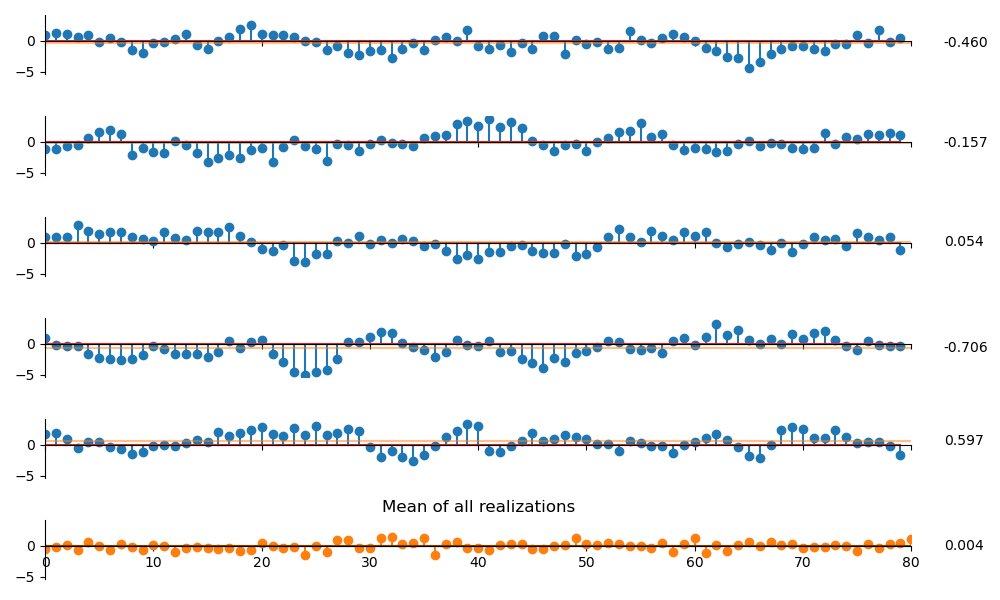
\includegraphics[width=12cm]{Figures/sp_ergodicity.png}
\caption{5 realizations of the stochastic process of the example \ref{ex:ergodic} (top), the average of 1000 realizations (bottom) and the averages of the represented samples (right). Because of the stationarity, the average signal (at the bootom) approaches a to a zero signal, which is mean of the process. Because of the ergodicity, time averages also approximate the mean.}
\label{fig:ergodicity}
\end{center}
\end{figure}
%%%%%%%%%%%%

%%%%%%%%%%%%%%%%%%%%%%%%%%%%%%%%%%%%%%%%%%%%%%%%%
\subsubsection{Ergodicity in the autocorrelation}

In a similar way, ergodicity is defined in autocorrelation. A WSS process $X_n$ is autocorrelation-ergodic if
\begin{equation}
\label{ec:autocorr_ergodic}
r_N = \frac{1}{2N+1}\sum_{m=-N}^{N} X_{m+n} X_m^*
\end{equation}
converges to $r_X[n]$ in squared mean. In general, $X_n$ is autocorrelation-ergodic if, for every value of $m$, the process $Z_n[m] = X_{m + n} X_m^*$ is mean-ergodic.





%%%%%%%%%%
%\appendix
%%%%%%%%%%
%
%%%%%%%%%%%%%%%%%%%%%%%%%%%%%%%%%%%%%
%\section{Teorema de Wiener-Khinchin}
%\label{sec:twk}
%
%Demostraremos aqu'i que \eqref{DEPvsR2} se reduce a \eqref{DEPvsRgeneral}. Para ello supondremos en primer lugar que la
%correlaci'on cruzada entre dos muestras $X(t)$ y $X(t+\tau)$ est'a acotada por un valor que solamente depende de la separaci'on entre
%ellas, de modo que
%\begin{equation}
%|r_X(t+\tau,t)| \le g(\tau)
%\label{eq:acontandorx}
%\end{equation}
%Asimismo, supondremos que la correlaci'on entre muestras decrece ``suficientemente r'apido'' al aumentar su separaci'on, de tal modo
%que
%\begin{equation}
%\int_{-\infty}^{\infty} g(\tau) d\tau < \infty 
%\label{eq:acontandorx2}
%\end{equation}
%lo que garantiza que $g(\tau)$, al ser no negativa, tiene transformada de Fourier.
%
%La integral doble \eqref{DEPvsR2} sobre el dominio cuadrado de anchura $T$ puede expresarse en funci'on de la integral sobre el dominio
%$-T\le t_2 \le T$, como
%\begin{eqnarray}
%S_X(\jw) 
%  &=& \lim_{T\rightarrow \infty}
%  \frac{1}{2T} \int_{-T}^T \int_{-\infty}^{\infty} r_X(t_2+\tau,t_2) e^{-\jw\tau} d\tau dt_2
%  \nonumber\\
%  &-& \lim_{T\rightarrow \infty}
%  \frac{1}{2T} \int_{-T}^T \int_{T-t_2}^{\infty} r_X(t_2+\tau,t_2) e^{-\jw\tau} d\tau dt_2
%  \nonumber\\
%  &-& \lim_{T\rightarrow \infty}
%  \frac{1}{2T} \int_{-T}^T \int_{-\infty}^{-T-t_2} r_X(t_2+\tau,t_2) e^{-\jw\tau} d\tau dt_2
%  \nonumber\\
%  &=& I_0(\jw) - I_1(\jw) - I_2(\jw)
%  \label{DEPvsR3}
%\end{eqnarray}
%donde hemos llamado, $I_0$, $I_1$ e $I_2$, a cada una de las tres integrales de la expresi'on anterior, siguiendo el orden en que
%aparecen. Demostraremos ahora que $I_1$ e $I_2$ se anulan. Para ello, podemos acotar el m'odulo de $I_1$ mediante
%\begin{eqnarray}
%|I_1(\jw)| &=& \left|\lim_{T\rightarrow \infty} 
%    \frac{1}{2T} 
%    \int_{-T}^T \int_{T-t_2}^{\infty} r_X(t_2+\tau,t_2) e^{-\jw\tau} d\tau dt_2
%  \right|
%  \nonumber\\
%  &\le& \lim_{T\rightarrow \infty} 
%  \frac{1}{2T} 
%  \int_{-T}^T \int_{T-t_2}^{\infty} |r_X(t_2+\tau,t_2)| d\tau dt_2
%  \nonumber\\
%  &\le& \lim_{T\rightarrow \infty} 
%  \frac{1}{2T} 
%  \int_{-T}^T \int_{T-t_2}^{\infty} g(\tau) d\tau dt_2
%\end{eqnarray}
%Asimismo, podemos calcular el l'imite de la expresi'on anterior descomponiendo la integral en suma de dos integrales sobre regiones
%disjuntas,
%\begin{eqnarray}
%  |I_1(\jw)| &\le& 
%  \lim_{T\rightarrow \infty} 
%  \frac{1}{2T} 
%  \int_{-T}^T \int_{T-t_2}^{T} g(\tau) d\tau dt_2
%  + \lim_{T\rightarrow \infty} 
%  \frac{1}{2T} 
%  \int_{-T}^T \int_{T}^{\infty} g(\tau) d\tau dt_2
%  \nonumber\\
%  &=& \lim_{T\rightarrow \infty} 
%  \frac{1}{2T} 
%  \int_{-T}^T \int_{T-t_2}^{T} g(\tau) d\tau dt_2
%  + \lim_{T\rightarrow \infty} 
%  \int_{T}^{\infty} g(\tau) d\tau
%  \label{DEPvsR4}
%\end{eqnarray}
%El segundo t'ermino se anula porque el intervalo de integraci'on tiende a 0. El primero se simplifica cambiando el orden de
%integraci'on respecto de las variables $\tau$ y $t_2$. Resulta, en tal caso,
%\begin{eqnarray}
%|I_1(\jw)| \le \lim_{T\rightarrow \infty} 
%  \frac{1}{2T} \int_0^T \int_{T-\tau}^{T} dt_2  g(\tau) d\tau
%  = \lim_{T\rightarrow \infty} 
%  \frac{1}{2} 
%  \int_0^T \frac{\tau}{T} g(\tau) d\tau
%  \label{DEPvsR5}
%\end{eqnarray}
%cuyo l'imite es cero. De un modo completamente an'alogo se concluye que $|I_2(\jw)|=0$. En consecuencia, \eqref{DEPvsR3} se reduce a
%\begin{eqnarray}
%S_X(\jw) 
%  = \lim_{T\rightarrow \infty}
%  \frac{1}{2T} \int_{-T}^T \int_{-\infty}^{\infty} r_X(t_2+\tau,t_2) e^{-\jw\tau} d\tau dt_2
%  \label{ITvsIInf4}
%\end{eqnarray}
%donde podemos intercambiar la integral y el l'imite al estar acotada $r_X(t_2+\tau,t_2)$ mediante \eqref{eq:acontandorx} y
%\eqref{eq:acontandorx2} , quedando finalmente
%\begin{eqnarray}
%S_X(\jw) = \int_{-\infty}^{\infty}
%  \lim_{T\rightarrow \infty}
%  \frac{1}{2T} \int_{-T}^T r_X(t_2+\tau,t_2) dt_2 
%  e^{-\jw\tau} d\tau 
%  \label{ITvsIInfFin}
%\end{eqnarray}
%y de aqu'i, sustiyendo la definici'on de $\overline{R}_X(\tau)$ seg'un \eqref{Rpromedio}, obtenemos \eqref{DEPvsRgeneral}.

